% #############################################################################
% This is Appendix A
% !TEX root = ../main.tex
% #############################################################################
\chapter{Pathological speech detection through pre-trained models}
\label{chapter:appendixA}

%\section{Introduction}
In the domain of speech therapy, and specifically paediatric speech therapy, advancements in \acp{SLT} hold significant promise by providing automated tools for assessing pronunciation quality and identifying pathological conditions. While the primary focus of this thesis was to improve \ac{ASR} for children, we also contributed to the identification of pathological conditions from speech for adult speakers. This annexe provides an overview of these contributions.


\section{Pathological speech detection using x-vector embeddings}
\subsection{Introduction}
Speech has been proposed as a valuable biomarker for detecting various diseases, including neurological conditions, mood disorders, and respiratory diseases \cite{hauptman2019identifying,botelho2019speech}. However, challenges such as temporal and financial constraints, lack of medical community awareness, ethical concerns, and patient privacy laws impede the acquisition of medical data, posing significant obstacles to the development of health-related speech-based classifiers, especially for deep learning models.

Most existing classifiers rely on \ac{KB} features, often limited in capturing subtle symptoms and variations in disease severity. To address this limitation, some studies focus on speaker representation models, such as Gaussian Supervectors and i-vectors. For instance, Hauptman \textit{et al.} \cite{hauptman2019identifying} proposed i-vectors for \ac{PD} classification, while Laaridh \textit{et al.} \cite{laaridh17_interspeech} applied the i-vector paradigm to predict dysarthric speech evaluation metrics. The motivation behind using these speaker representations lies in their ability to model speaker variability, which should also include disease symptoms \cite{hauptman2019identifying}.

X-vectors are discriminative \ac{DNN}-based speaker embeddings, surpassing i-vectors in tasks like speaker and language recognition \cite{snyder2018x}. Despite initial doubts about the usability of such discriminative representations for disease detection as they have been trained on general datasets without diseased patients, recent studies have demonstrated their effectiveness. Indeed, x-vectors have been successfully applied to paralinguistic tasks such as emotion recognition \cite{pappagari2020x}, obstructive sleep apnea detection \cite{perero2019modeling}, and as a complement feature for Alzheimer’s disease detection \cite{zargarbashi2019multi}. In our work \cite{botelho2020pathological}, we investigated the hypothesis that speaker characteristics embedded in x-vectors, obtained from a single network trained for speaker identification using general data, contain sufficient information for the detection of multiple diseases. Furthermore, we aimed to assess whether this information persists even in the presence of language mismatch training, a phenomenon previously observed in speaker recognition \cite{snyder2017deep}. Specifically, we employ the x-vector model as a feature extractor to train \ac{SVM} for detecting two speech-affecting diseases: \ac{PD} and  \ac{OSA}.

\subsection{Speaker embeddings: i-vector and x-vector}
Speaker embeddings serve as fixed-length representations of variable-length speech signals, capturing essential information about the speaker. Traditional methods, such as Gaussian Supervectors \cite{kenny2007joint} derived from \ac{MAP}-adapted \ac{GMM-UBM} \cite{reynolds2000speaker} and i-vectors \cite{dehak2010front}, have been fundamental in speaker recognition.

I-vectors, until recently considered as state-of-the-art, extend the \ac{GMM} Supervector approach by modelling total variability as a low-rank space through factor analysis. Hauptman \textit{et al.} observed that i-vectors, while capturing total variability and speaker variability, also encompass information about speech disorders \cite{hauptman2019identifying}. For classification, they used reference i-vectors for healthy and \ac{PD} populations.

In contrast, x-vectors, proposed as an alternative to i-vectors, aim to discriminate between speakers by modelling specific characteristics. Unlike i-vectors, x-vectors exhibit robustness to data variability and domain mismatches, requiring shorter temporal segments for optimal performance. Typically, the x-vector system comprises three main blocks: \ac{TDNN} layers operating at the frame level, a statistical pooling layer for temporal aggregation (employing an attentive mechanism for importance weighting), and fully connected (Dense) layers for x-vector extraction.

\subsection{Experimental setup}
In our experiments, we used four corpora to determine the presence or absence of \ac{PD} and \ac{OSA}. Using specifically one of the European Portuguese corpus to train the i-vector and x-vector extractors. For each disease-related dataset, we compared three sets of features: \ac{KB} features, i-vectors, and x-vectors. All disease classifications were conducted using a \ac{SVM} classifier using leave-one-speaker-out cross-validation as an alternative to partitioning the corpora into train, development and test sets. Further details on the corpora, data representations, and classification method are provided below in Section \ref{sec:corpora_xvector_path}.

Additionally, our classification processes operate at the segment level, assigning speakers a final classification through a weighted majority voting mechanism. With this approach, predictions obtained for each segment uttered by the speaker are weighted based on the corresponding number of speech frames they contain.

\subsubsection{Corpora}
\label{sec:corpora_xvector_path}
In this section, we provide a description of the four datasets employed in our study. All utterances were segmented into 4-second-long segments using overlapping windows with a 2-second shift. Further details about each of these datasets can be found in Table \ref{tab:xvect_data}.

\begin{itemize}
  \item \textbf{Speaker Recognition:} Portuguese (PT-EASR) Corpus is a subset of the EASR (Elderly Automatic Speech Recognition) corpus \cite{hamalainen2014easr}. It comprises recordings of European Portuguese read sentences and was used for training both i-vector and x-vector models for a speaker recognition task. The dataset encompasses speakers aged from 24 to 91, with 91\% falling within the 60-80 age range. This specific age distribution was chosen with the intention of generating reliable speaker embeddings for this age group, particularly relevant to the diseases addressed in our study. The corpus was partitioned into training, development, and test sets in a ratio of 0.70:0.15:0.15, respectively.

  \item \textbf{\ac{PD} Detection:} The Portuguese \ac{PD} (PPD) Corpus, a subset of the FraLusoPark corpus \cite{pinto2016dysarthria} was employed. This corpus includes speech recordings of both French and European Portuguese healthy volunteers and \ac{PD} patients. For our experiments, we selected utterances of European Portuguese speakers reading prosodic sentences only.

  \item \textbf{Spanish \ac{PD} Detection}: We use the Spanish \ac{PD} (SPD) Corpus corresponds to a subset of the New Spanish Parkinson’s Disease Corpus, collected at the Universidad de Antioquia, Colombia \cite{orozco2014new}. For this experiment, we only used the read sentences subset. This corpus serves the purpose of investigating whether x-vector representations trained in one language (European Portuguese) can generalise effectively to another language, namely Spanish.
  
  \item \textbf{ \ac{OSA} Detection:} The corpus used in this experiment, is an extended version of the Portuguese Sleep Disorders (PSD) corpus \cite{botelho2019speech}. This corpus includes three tasks in European Portuguese: reading a phonetically rich text, reading sentences recorded during a cognitive load assessment task and spontaneous descriptions of an image. 
\end{itemize}


\begin{table}[h]
  \centering
  \begin{tabular}{cccccc}
  \hline
  Language & Task & Group & Speakers & Segments & Duration (h) \\
    \hline
  \multirow{5}{*}{PT} & Spk. Rcg. & - & 919 & 290,690 & 171.81  \\ \cline{2-6}
  & \multirow{2}{*}{PD} & Patient & 75 & 1,838 & 1.24 \\
  & & Control & 65 & 1,527 & 1.07 \\ \cline{2-6}
  & \multirow{2}{*}{OSA} & Patient & 30 & 1,793 & 1.10 \\
  &  & Control & 30 & 1,702 & 1.05 \\
  \hline
  \multirow{2}{*}{SP} & \multirow{2}{*}{PD} & Patient & 50 & 661 & 0.49 \\
  & & Control & 50 & 655 & 0.50 \\

  \hline
  \end{tabular}
  \caption{Detailed description of the different datasets used for pathology detection with speakers, segments and number hours information}
  \label{tab:xvect_data}
  \end{table}
  

\subsubsection{Knowledge based features}
For \ac{PD} classification, the \ac{KB} feature set was proposed by Pompili \textit{et al.} \cite{pompili2017automatic} and comprises 36 features from the eGeMAPS \cite{eyben2015geneva}, along with the mean and standard deviation of 12 \acp{MFCC} and log-energy. Additionally, the set includes the first and second derivatives of these coefficients, resulting in a 114-dimensional feature vector.

In the case of \ac{OSA} classification, the \ac{KB} feature set, as proposed in Botelho \textit{et al.} \cite{botelho2019speech}, includes the mean of 12 \acp{MFCC}, along with their first and second order derivatives, and 48 linear prediction cepstral coefficients. The set also covers the mean and standard deviation of the frequency and bandwidth of formant 1, 2, and 3, as well as the mean and standard deviation  of Harmonics-to-noise ratio, jitter, F0 at percentiles 20, 50, and 100, and mean and standard deviation  values for all frames and only voiced frames of Spectral Flux. All \ac{KB} features were extracted using openSMILE \cite{eyben2013recent}.

\subsubsection{Speaker embeddings}
\begin{table}[h]
  \centering
  \begin{tabular}{ccccc}
  \hline
  Layer & Contex & Total Contex & In $\times$ Out \\
  \hline
  TDNN1 & $[t-2, t+2]$ & 5 & $5F \times 256$ & \\
  TDNN2 & $\{t-2, t, t+2\}$ & 9 & $768 \times 256$ & \\
  TDNN3 & $\{t-3, t, t+3\}$ & 15 & $768 \times 256$ & \\
  TDNN4 & $\{t\}$ & 15 & $256 \times 256$ & \\
  TDNN5 & $\{t\}$ & 15 & $256 \times 512$ & \\
  stats pooling & $[0, T)$ & $T$ & $512T \times 1024$ & \\
  Dense 6 & $\{0\}$ & $T$ & $1024 \times 512$ & \\
  Dense 7 & $\{0\}$ & $T$ & $512 \times 512$ & \\
  softmax & $\{0\}$ & $T$ & $512 \times S$ & \\
  \hline
  \end{tabular}
  \caption{X-vector network architecture, used to train the x-vector embedding extractor with the PT-EASR dataset}
  \label{tab:xvect_description}
  \end{table}
  In the i-vector system, 19 \acp{MFCC} plus log-energy are given as input with non-speech frames removed using energy-based \ac{VAD}. Utterances are modelled with a 512-component full-covariance \ac{GMM}, resulting in 180-dimensional i-vectors. The entire process is implemented using Kaldi \cite{kaldi} over the PT-EASR corpus.

  For x-vectors, the network architecture is detailed in Table \ref{tab:xvect_description}, and x-vectors are extracted at the $6^{th}$ layer (Dense 6). Using 24-dimensional \ac{fbanks} as input features. The non-speech frames were removed using energy-based \ac{VAD}. This network was trained, using Pytorch \cite{paszke2019pytorch}on the PT-EASR corpus for speaker identification, using 100 epochs, cross-entropy loss, a learning rate of 0.001, a learning rate decay of 0.05 with a 30-epoch period, a batch size of 512, and a dropout value of 0.001.

\subsection{Results}
\begin{table}[h]
  \begin{tabular}{cc|ccc|ccc|ccc} \hline
                            &     & \multicolumn{3}{c|}{PD - Portuguese} & \multicolumn{3}{c|}{OSA}                      & \multicolumn{3}{c}{PD - Spanish} \\ \hline
  Features                  &     & Prec.        & Recall           & F1 Score        & Prec.     & Recall        & F1 Score      & Prec.       & Recall         & F1 Score       \\ \hline
  \multirow{2}{*}{KB}       & Seg & 64.5             & 64.6             & 64.5            & 64.8          & 64.9          & 64.8          & \textbf{79.0}   & \textbf{79.0}  & \textbf{79.0}  \\
                            & Spk & 72.2             & 72.3             & 72.1            & \textbf{82.0} & \textbf{81.7} & 81.6          & \textbf{87.1}   & \textbf{87.0}  & \textbf{87.0}  \\ \hline
  \multirow{2}{*}{i-vector} & Seg & 66.6             & 66.6             & 66.6            & 65.6          & 65.6          & 65.6          & 75.7            & 75.7           & 75.7           \\
                            & Spk & \textbf{75.6}    & \textbf{75.7}    & \textbf{75.6}   & 72.3          & 75.0          & 75.0          & 85.1            & 85.0           & 85.0           \\ \hline
  \multirow{2}{*}{x-vector} & Seg & \textbf{66.7}    & \textbf{66.8}    & \textbf{66.7}   & \textbf{73.3} & \textbf{73.3} & \textbf{73.3} & 77.2            & 77.2           & 77.1           \\
                            & Spk & 74.4             & 74.5             & 74.3            & 81.7          & \textbf{81.7} & \textbf{81.7} & 86.0            & 86.0           & 86.0 \\ \hline    
  \end{tabular}
  \caption{Precision, recall and F1 score results of the different pathologies detection with KB and speaker embeddings}
  \label{tab:xvect_results}
  \end{table}
The results of the different tasks are summarised in Table \ref{tab:xvect_results}. For \ac{PD} with Portuguese data, the findings indicate that speaker representations learned from out-of-domain data surpass the performance of \ac{KB} features. This supports our hypothesis that speaker embeddings not only capture information about the speaker but also model symptoms of the disease that \ac{KB} features may fail to include.

It is notable that x-vectors and i-vectors yield very similar results, with a slight advantage for x-vectors at the segment level and slightly better results for i-vectors at the speaker level. This observation suggests that while x-vectors offer stronger representations for short segments, i-vectors may perform better for longer segments. The application of a majority vote weighted by the duration of speech segments may favour the i-vector approach at the speaker level.

In the context of the \ac{OSA} task, x-vectors demonstrate superior performance compared to all other approaches at the segment level. Notably, they significantly showed around 8\% improvement over \ac{KB} features, providing further support for our hypothesis. However, it is essential to highlight that both x-vectors and i-vectors perform similarly at the speaker level. Interestingly, i-vectors, in this scenario, perform less effectively than \ac{KB} features. One possible explanation could be attributed to the fact that the PSD corpus incorporates tasks, such as spontaneous speech, which diverge from the read sentences included in the corpus used to train the i-vector and x-vector extractors. These tasks might be considered out-of-domain, which would explain why x-vectors outperform the i-vector approach.

The objective of the \ac{PD} Spanish experiment was to evaluate the efficacy of x-vectors trained in one language when applied to disease classification in a different language. Our findings reveal that \ac{KB} features outperform both speaker representations, possibly due to the language mismatch between the Spanish \ac{PD} corpus and the European Portuguese training corpus. However, it is noteworthy that, akin to the previous task, x-vectors demonstrate the ability to surpass i-vectors in an out-of-domain corpus.

To conclude, our experiments conducted on the European Portuguese datasets substantiate the hypothesis that speaker embeddings encompass pertinent information for disease detection. Notably, we identified evidence indicating that these embeddings capture information not represented by \ac{KB} features, validating the efficacy of our approach. Additionally, the observations suggest that x-vectors outperform i-vectors in tasks where the domain does not align with the training data, such as verbal task mismatch and cross-lingual experiments. This underscores the potential of x-vector embeddings as formidable alternatives to \ac{KB} feature sets for the detection of \ac{PD} and \ac{OSA}.


\section{The INESC-ID Multi-Modal System for the ADReSS 2020 Challenge}
\subsection{Introduction}
Later, we proposed to extend the aforementioned work by classifying \ac{AD} \cite{pompili2020inesc}. Indeed, existing studies have explored various approaches, including the use of syntactic or semantic features, plain acoustic methods, and combinations of speech and lexical parameters. However, the diversity in datasets and methodologies makes it challenging to compare these studies. To address this, the Alzheimer's Dementia Recognition through Spontaneous Speech (ADReSS) challenge was introduced, providing a common, statistically balanced, and acoustically enhanced dataset for researchers to test their approaches. In this work, we introduced a multi-modal system where both acoustic and textual feature embeddings were used for automatically distinguishing \ac{AD} patients
from healthy individuals. 

In the literature, studies focused on hand-crafted temporal and acoustic parameters from speech or linguistics or a fusion of both. For example, a study analysed temporal speech features \cite{konig2015automatic}. Another work employed over 350 features to capture lexical, syntactic, grammatical, and semantic phenomena from transcriptions of a picture description task \cite{fraser2016linguistic}. Finally, Gosztolya \textit{et al.} consider a set of feature including in conjunction demographic, acoustic, and linguistic features \cite{gosztolya2019identifying}.

More recently, a shift towards advanced architectures has been observed to overcome the limitations of traditional methods. For instance, Warnita \textit{et al.} \cite{warnita18_interspeech} used a gated \ac{CNN} on acoustic data, while Karlekar \textit{et al.} \cite{karlekar-etal-2018-detecting} explored linguistic impairments with \ac{CNN}, \acp{RNN}, and a combination. Finally, some work introduced a multi-modal feature embedding approach, based on n-gram, i-vector and x-vectors \cite{zargarbashi2019multi}.

Our work differs from previous studies in two aspects. First, by using contextual embedding vectors for text data, feeding into two systems: one employing Global Maximum pooling and bidirectional \ac{LSTM}-\acp{RNN} architectures, and the other based on statistical computation of sentence embeddings. Secondly, for audio, we use \ac{DNN} speaker embeddings extracted from pre-trained models. To the best of our knowledge, this is the first work which jointly uses automatically learned representations for both audio and textual data. Additionally, our approach is simpler and does not require training deep architectures.

\subsection{Corpus}
\begin{table}[h]
  \begin{center}
   \begin{tabular}{c|ccc}
    \hline
                    & \multicolumn{2}{c}{Train} & Test       \\ \cline{2-4}
                    & \textit{Control}     & \textit{AD}          & -          \\ \hline
  Audio Full        & 55min46s    & 1h14min     & 1h06min    \\
  Audio chunks      & 30min11s    & 26min31s    & 26min32s   \\
  \# Words (unique) & 6097 (567)  & 5494 (552)  & 5536 (602) \\ \hline
  \end{tabular}
  \caption{Statistical information on the ADReSS corpus}
  \label{tab:adress_data}
  \end{center}
  \end{table}
The ADReSS dataset comprises speech recordings and annotated transcriptions from 156 subjects, including 78 \ac{AD} patients and 78 healthy control speakers. The data is split into training (108 subjects) and test (48 subjects) sets. Participants provided descriptions of the Cookie Theft picture from the Boston Diagnostic Aphasia Examination \cite{goodglass2001bdae}. Speech recordings were segmentated using \ac{VAD} and normalised \cite{luz2020alzheimer}. The dataset contained both fully enhanced audio and normalised audio chunks. Our approach used both audio and transcriptions available. The transcriptions were annotated with disfluencies, filled pauses, repetitions and other complex events. The transcriptions contained 17,127 words, including 1,009 unique words. Additional details on the duration and size of the ADReSS dataset are provided in Table \ref{tab:adress_data}.
\subsection{Proposed system}
\begin{figure}[h]
  \begin{center}
  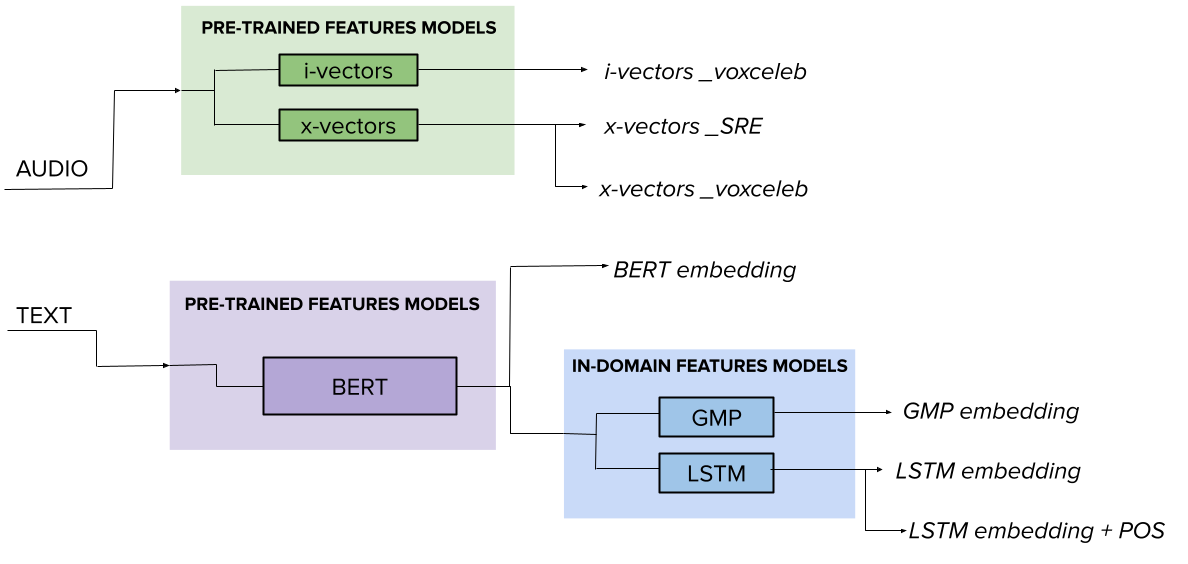
\includegraphics[scale=0.35]{imgs/ADReSS.png}  
  \caption{Overview of the multimodal system based on embedding approaches}
  \label{fig:adress_overview}
  \end{center}
\end{figure}
Our multi-modal framework, illustrated in Figure \ref{fig:adress_overview}, is based on the independent generation of acoustic and textual feature embeddings. Subsequently, we conduct an early fusion of the output of the two systems to create a single feature vector encapsulating a condensed representation of both speech and language characteristics of the utterance. The final classification is carried out using an \ac{SVM} classifier with a linear kernel. Further details of the two systems used in our experiments will be provided in the following sections.
\subsubsection{Acoustics modality}
The acoustic system incorporates i-vectors and x-vectors. Taking into consideration the small size of the ADReSS dataset, we preferred to use already existing pre-trained models to produce the acoustic feature embeddings, rather than training them using in-domain challenge data. For the x-vectors framework, both the SRE and Voxceleb models were employed. The SRE model was primarily trained on telephone and microphone speech using data from the Switchboard corpus, Mixer 6, and NIST SREs \cite{snyder2018x}. The Voxceleb model was trained on augmented VoxCeleb 1 and VoxCeleb 2 datasets, encompassing speech from speakers with diverse ethnicities, accents, professions, and ages \cite{snyder2018x,nagrani17_interspeech}. The VoxCeleb dataset was also used to build the i-vectors pre-trained model used in our experiments.

For all these pre-trained models, the inputs included 23 and 30-dimensional \acp{MFCC} extracted with the Kaldi toolkit \cite{kaldi} and non-speech frames were filtered out using \ac{VAD}. For x-vectors, 512-dimensional embeddings were extracted, while i-vectors, based on \ac{GMM-UBM}, were of dimension of size 400.

\subsubsection{Linguistic modality}
For the linguistic modality, we used two distinct methods to extract textual feature embeddings. Firstly, we explored training deep architectures on a relatively small corpus with dimensions of the same range as the one used in this challenge. Then, we compare this approach with a less data-intensive method based on extracting sentence embeddings using a pre-trained model. Both strategies use contextual word embeddings as input but produce different types of learned representations as output. In order to integrate information from linguistics in conjunction with the acoustic systems, the trained architectures were employed to extract linguistic features before the final classification layer. In this way, we obtain a single 768-dimensional feature vector for an entire description. The sentence embedding approach, on the other hand, provides a single 768-dimensional vector for each sentence of a description.

For both approaches, the initial pipeline step involved normalising the text data of the ADReSS dataset. Clean transcriptions were encoded into 768-dimensional context embedding vectors using a pre-trained English BERT model with 12 layers and 768 hidden units \cite{Bert}. Then, the first system is derived from the ComParE2020 Elderly Challenge baseline \cite{schuller2020interspeech}, involved training three neural models on top of contextual word embeddings: (i) a Global Maximum pooling, (ii) a bidirectional \ac{LSTM} (biLSTM) with an attention module, and (iii) the second model augmented with part-of-speech (POS) embeddings. The loss was evaluated during training on the development set.

The second system does not require an additional training phase, as representations are extracted from a pre-trained model to directly characterise linguistic deficits in \ac{AD}. Contextual word embeddings obtained for each word were used to compute fixed-size embedding vectors for each sentence by averaging the second to twelfth hidden layers of each word.

\subsection{Results}
\begin{table}[h]
  \begin{center}
  \begin{tabular}{lcccc}
  \hline
  & \multicolumn{1}{l}{\textbf{Accuracy}} & \multicolumn{1}{l}{\textbf{Precision}} & \multicolumn{1}{l}{\textbf{Recall}} & \multicolumn{1}{l}{\textbf{F1 Score}} \\
  \hline
  x-vectors\_Vox           & 0.6818                               & 0.6834                                & 0.6919                             & 0.6812                               \\
  x-vectors\_SRE              & \textbf{0.7273}                               & \textbf{0.7273}                                & \textbf{0.7273}                             & \textbf{0.7273}                               \\
  i-vectors\_Vox          & 0.6818                               & 0.7292                                & 0.6818                             & 0.6645                               \\
  i-vectors\_Vox\_x-vectors\_Vox & 0.7273                               & 0.7273                                & 0.7273                             & 0.7273                               \\
  i-vectors\_Vox\_x-vectors\_SRE      & 0.7273                               & 0.7351                                & 0.7273                             & 0.7250                                \\
  \hline
  \end{tabular}
  \caption{Results of different acoustic approaches on the development set}
  \label{tab:adress_acoustics}    
\end{center}
\end{table}

The results obtained using the different acoustic feature embeddings are summarised in Table \ref{tab:adress_acoustics}. Different independent models were explored, and an early fusion of the best acoustic results was performed. The x-vectors Voxceleb model generally achieved lower classification accuracy. However, when combining i-vectors and x-vectors both trained with VoxCeleb, the accuracy was comparable to x-vectors only trained on the SRE corpus, which represents the best acoustic result on the development set. These outcomes are slightly lower than those reported in similar works in the literature \cite{warnita18_interspeech,zargarbashi2019multi}. However, our approach is distinct from these previous studies as we use a smaller dataset and do not rely on \ac{DNN} training. To validate these results on the test set, we select the acoustic feature embeddings extracted from the pre-trained x-vectors SRE model for evaluation.
\begin{table}[h]
  \begin{tabular}{lcccc}
  \hline
& \multicolumn{1}{l}{\textbf{Accuracy}} & \multicolumn{1}{l}{\textbf{Precision}} & \multicolumn{1}{l}{\textbf{Recall}} & \multicolumn{1}{l}{\textbf{F1 Score}} \\ \hline
  Global Max Pool. & 0.7727                               & 0.7947                                & 0.7728                             & 0.7684                               \\
  LSTM-RNNs        & 0.8182                               & 0.8182                                & 0.8182                             & 0.8182                               \\
  LSTM-RNNs Pos    & 0.8636                               & 0.8667                                & 0.8637                             & 0.8634                               \\
  GMax/LSTM-RNNs/LSTM-RNNs-Pos                   & \textbf{0.9091}                               & \textbf{0.9091}                                & \textbf{0.9091}                             & \textbf{0.9091}  \\  
  %\textit{\textbf{Sentence emb.}  }                  & 0.6930                               & 0.6864                                & 0.6903                             & 0.6873  \\
  \textit{\textbf{Sentence emb. - maj. vote}}                    & 0.7727                               &0.7947                & 0.7728                           & 0.7684
  \\ \hline
  \end{tabular}
  \caption{Results of different linguistic approaches on the development set}
  \label{tab:res_dev_ling}
  \end{table}

  The results obtained with our various linguistic systems are shown in Table \ref{tab:res_dev_ling}, presenting the performance for features trained with three neural models, their fusion, and the sentence embedding approach. For the sentence embedding approach, the accuracy uses a majority voting strategy over the entire description. Our best classification result attained an accuracy of 90.91\% on the development set using the fusion of the linguistic feature sets generated by the three neural models. Comparing this result with the one obtained by sentence embeddings, we acknowledge that neural models outperform simpler strategies even with constrained training data. This was surprising and in contradiction with similar experiments performed with the acoustic system. We hypothesise that the large amount of contextual information provided by the BERT model is helpful in overcoming the limited size of the ADReSS dataset. Nevertheless, we suspect that the high accuracy attained with neural models may be too optimistic, due to the fact of having used the development set both for testing and evaluating the model’s loss. Thus, in spite of their lower outcome, the sentence embedding approach is selected as one of the systems to be evaluated on the test set. In fact, on the one hand, we think that they may represent a more reliable system, since do not require additional training. On the other hand, we also observe that they achieve higher classification scores when compared with a similar approach based on GloVe embeddings \cite{mirheidari2018detecting}, thus corroborating our decision.

  For a comprehensive evaluation of speech and language impairments in \ac{AD}, we performed an early fusion of the best results from both the acoustic and linguistic systems. This involved merging x-vectors with linguistic feature sets from three neural models. However, the results of the development set using this extended feature set did not yield additional improvements. Despite this, we selected the combined system as our primary choice for evaluation.

  \begin{table}[h]
    \begin{center}
    \begin{tabular}{llcccc}
    \hline
     & \textbf{Class} & \multicolumn{1}{l}{\textbf{Accuracy}} & \multicolumn{1}{l}{\textbf{Precision}} & \multicolumn{1}{l}{\textbf{Recall}} & \multicolumn{1}{l}{\textbf{F1 Score}} \\ 
                                         \hline
    Fusion of system   &  AD             & \multirow{2}{*}{\textbf{0.8125}}                     & 0.9412                                 & 0.6667                              & 0.7805                                \\
   & non-AD         &                                       & 0.7419                                 & 0.9583                              & 0.8364                                \\
    %                                     & Avg.           & \textbf{0.8125}                       & \textbf{0.8415}                        & \textbf{0.8125}                     & \textbf{0.8085}                       \\
    Sentence embedding &  AD             &  \multirow{2}{*}{\textbf{0.7292}}                                    & 0.8235                                 & 0.5833                              & 0.6829                                \\
     & non-AD         & \multicolumn{1}{l}{}                  & 0.6774                                 & 0.8750                              & 0.7636                                \\
    %                                     & Avg.           & 0.7292                                & 0.7505                                 & 0.7292                              & 0.7233                                \\
    x-vectors\_SRE     & AD             & \multirow{2}{*}{\textbf{0.5417}}                                      & 0.5417                                 & 0.5417                              & 0.5417                                \\
    & non-AD         & \multicolumn{1}{l}{}                  & 0.5417                                 & 0.5417                              & 0.5417                                \\ \hline
    %                                     & Avg.           & 0.5417                                & 0.5417                                 & 0.5417                              & 0.5417    \\ \hline
    \end{tabular}
    \caption{Results of different acoustic and linguistic approaches on the test set}
    \label{tab:adress_test}  
  \end{center}
    \end{table}


  For the evaluation, three systems were submitted: (i) a fusion of the best results from linguistic and acoustic systems, (ii) sentence embeddings, and (iii) the best acoustic system. Results on the test set, presented in Table \ref{tab:adress_test}, showed a consistent drop in performance compared to the development set, even for systems not requiring a training phase. The first system achieved the best result with an accuracy of 81.25\%, indicating the capability of deep architectures with contextual word embeddings to overcome dataset limitations. The acoustic system alone yielded the lowest accuracy at 54.17\%, suggesting room for improvement in adapting acoustic pre-trained models, for example, to better model elderly speech characteristics.



\section{Transfer Learning-Based Cough Representations for Automatic Detection of COVID-19}
\subsection{Introduction}
Finally, in our final work presented in this annexe \cite{SoleraUrea2021TransferLC}, we further extend the idea of using pre-trained representation to automatically detect COVID-19 from cough recordings. Indeed, the COVID-19 respiratory disease was declared a pandemic by the World Health Organisation in March 2020, with profound personal, societal, and economic consequences. Clinical diagnosis primarily relies on RT-PCR and antigen tests, but these methods have drawbacks such as significant costs, intrusive sample collections, and delays in diagnosis due to laboratory saturation. To address these challenges, there was a growing interest in developing reliable, cost-effective, immediate, and user-friendly tools to optimise screening campaigns for healthcare operators, institutions, and companies.

In our work, we contributed to the ComParE 2021 COVID-19 Cough Sub-challenge \cite{schuller21_interspeech}. Firstly, we employed transfer learning to develop COVID-19 classification subsystems using deep cough representation extractors, including \ac{TDNN-F} and \ac{CNN} embeddings, as well as \ac{PASE}+ features. Secondly, we integrate individual decisions from the three experts into a calibrated decision-level fusion system. This ensemble of expert subsystems, relying on cough representations, aims to generate well-calibrated log-likelihood scores across various operating points. The resulting output can be readily interpreted by human experts and seamlessly incorporated into the decision-making process.

Current research on the automatic detection of COVID-19 from speech or respiratory sounds builds on prior studies demonstrating the distinct effects of various respiratory diseases on these sounds. This approach has proven effective in detecting pertussis, asthma, pneumonia, and tuberculosis, among others \cite{pramono2016cough}. While conclusive evidence is still pending for COVID-19, preliminary findings suggest specific signatures of COVID-19 in coughs and speech that could potentially enable detection even in apparently asymptomatic individuals and differentiate it from other common respiratory diseases. Given the limited availability of labelled COVID-19 data, many approaches rely on transfer learning, data augmentation, and class balancing techniques.

The majority of previous work in this domain relies on \acp{CNN}. For instance, a pre-trained VGGish model \cite{Hershey2017} was employed as a generic audio feature extractor \cite{Chloe2020}. Other works fine-tune \acp{CNN} initially trained for cough detection for the purpose of COVID-19 detection \cite{Bagad2020,Imran2020}. Ensemble models incorporating both \acp{DNN} and \acp{CNN}, directly trained from scratch for COVID-19 detection, have also been proposed \cite{Chaudhari2021}. Additionally, certain studies  \cite{Han2021} leverage information about self-reported symptoms, encoding them as one-hot vectors and combining them either at the feature- or decision levels with traditional speech features.

\subsection{Corpora}
In this work, we used two datasets: the COVID-19 COUGH (C19C) corpus, provided in the ComParE 2021 COVID-19 Cough Sub-Challenge \cite{Chloe2020,Han2021} for evaluation, and the COUGHVID corpus \cite{Orlandic2020}, employed for training and fine-tuning transfer learning-based cough representation extractors. Silence segments were eliminated from both datasets using \ac{VAD}.

The COVID-19 COUGH (C19C) corpus is a subset of the Cambridge COVID-19 Sound database \cite{Chloe2020,Han2021}, consisting of 725 cough recordings from 397 participants with self-reported COVID-19 status labels (positive/negative). The corpus is distributed into a train (71 positives/215 negatives), development (48 positives/183 negatives), and a blind test set (208 samples) with gender-balanced subsets. 

In our preliminary analysis, it was observed that some files had a reduced bandwidth of 4 k\ac{Hz}, potentially corresponding to samples originally recorded at 8 k\ac{Hz}. Namely, 13, 8 and 8 narrow-band files were detected in the train, development and test subsets, respectively. This condition certainly reflects the reality of many real-world applications. However, we noticed that all the narrow-band recordings in the train and development subsets correspond to the COVID-19-positive class. To address this, a second version of the dataset, denoted as ``$\text{C19C}_{fullband}$", was created by removing narrow-band recordings from the original train and development subsets. This resulted in 273 samples in the training subset (58 positives/215 negatives) and 223 in the development subset (40 positives/183 negatives), while the test subset remained unchanged for consistent challenge evaluation conditions.

The COUGHVID corpus \cite{Orlandic2020} is a publicly open dataset consisting of non-curated recordings performed using lossy codification. In addition, the dataset includes a variety of conditions such as sampling rate, bandwidth, number of channels, and quality. Volunteers recorded their coughs and reported their COVID-19 status (positive/symptomatic/healthy), age, gender, and medical condition.
The dataset comprises 27,550 recordings, with 15,125 classified as coughs by an automatic cough detector. Of these, 10,763 have self-provided gender and COVID-19 status annotations, including 680 COVID-19 positives (395 male/285 female), 8,270 healthy (5,632 male/2,638 female), and 1,813 symptomatic (1,114 male/699 female). Additionally, a small fraction of the dataset was annotated by expert pulmonologists with information on various aspects, such as type of cough, presence of audible symptoms, diagnosis, and severity.

\subsection{Proposed system}

\subsubsection{TDNN-F embedddings}
X-vector embeddings are currently regarded as state-of-the-art speaker representations, surpassing other proposed representations like d-vectors and i-vectors. Motivated by the results of the two previous works mentioned earlier in this annexe, this study explores the applicability of x-vector-like embeddings to coughs, aiming to encode relevant information about the cough signal for medical insights.
The X-vector extractor is implemented using \ac{TDNN-F} architecture as proposed for in previous work of speaker recognition \cite{villalbaSRE182020}. Cough embeddings are 128-dimensional vectors obtained at the output of the final dense layer. The network undergoes two-stage training: initially, an age estimation and gender classification using a subset of the COUGHVID dataset was performed, and subsequently fine-tuning with expert-annotated data for tasks closely related to COVID-19 classification. These tasks include cough type, presence of dyspnea, presence of wheezing, diagnosis, and severity. The reason behind this fine-tuning step is the fact that these tasks are much closer to COVID-19 classification than age and gender. The given input features to the model consist of 30 \acp{MFCC} computed every 10 ms from 25 ms-length frames, following the \textit{egs/voxceleb/v2} Kaldi recipe \cite{kaldi}.

\subsubsection{CNN embedddings}
Reported \ac{CNN}-based approaches for COVID-19 detection suffer from some limitations such as the use of \acp{CNN} as generic audio feature extractors without task-specific tuning or relying on relatively small datasets for training. In contrast, our work addresses these limitations by leveraging transfer knowledge from the VGGish model, originally trained on a large corpus for audio classification, and subsequently fine-tuned for COVID-19 detection using the COUGHVID dataset.

The VGGish model \cite{Hershey2017}, is an adaptation of the VGG network \cite{Simonyan2015} for audio classification. It consists of four blocks of convolutional and pooling layers, followed by fully-connected layers and an output layer. In this work, a simplified version of the model is used and was pre-trained using 5.4 million hours of YouTube data. For our experiments, we used two different settings. In the first setting, the model serves as a pre-trained generic feature extractor with weights directly loaded from the original model. In the second setting, the model is fine-tuned for COVID-19 detection using a balanced subset of the COUGHVID dataset. The input to the VGGish network is log Mel-spectrogram features computed every 0.24 s from 0.96 s-length segments and the resulting embeddings are 256-dimensional vectors.

When fine-tuning, the last two layers, namely the dense and output layers, are replaced to facilitate training with limited data, with their weights initialised randomly. The entire \ac{CNN} is fine-tuned for 150 epochs using cross-entropy loss, the Adam optimiser with a learning rate of $10^{-5}$, and a batch size of 64. The fine-tuning is conducted on a balanced subset of the COUGHVID dataset, consisting of 680 positive and 680 negative cough recordings, with 80\% used for training and 20\% for development.

\subsubsection{PASE+ embedddings}
Our study incorporates the problem-agnostic speech encoder model, \ac{PASE}+ \cite{Pascual2019,Ravanelli2020}, where targets are learned directly from the
signal in an unsupervised manner. \ac{PASE}+ features are derived from a shared encoder with a SincNet-based layer \cite{Sincnet}, seven convolutional blocks, and a Quasi-\ac{RNN} layer. The encoder output is connected to twelve workers, each designed for specific tasks like reconstruction of the waveform, \ac{LPC}, \acp{MFCC}, prosody, \ac{fbanks}, gamma tone, and some binary discrimination tasks. Two \ac{PASE}+ extractors were used: one pre-trained on Librispeech \cite{librispeech} and another trained from scratch on COUGHVID data. Both are trained for 150 epochs, creating 256-dimensional feature vectors for each frame every 10 ms.

\subsubsection{COVID-19 condition classification}
The key aspect of our study is to employ transfer learning to address the limited COVID-19 data for training. For classification, three \acp{SVM} were used respectively on \ac{TDNN-F} embeddings, \ac{CNN} embeddings, and \ac{PASE}+ features. In practice, \ac{TDNN-F} embeddings are directly input to the \ac{SVM}. \ac{CNN}-based embeddings are derived from cough segments and subjected to majority voting for the final decision. \ac{PASE}+ features are averaged across the sequence and fed to the \ac{SVM} classifier. The \acp{SVM} are trained on both the C19C and $\text{C19C}_{fullband}$ datasets, exploring various kernels, data normalisations, and class balancing methods. Hyperparameters are optimised through grid-search on development subsets, and linear logistic regression is applied to combine system decisions with scaling factors. The regression approximates log-likelihood ratios, thus, a theoretically determined decision threshold can be used for making hard decisions.

\subsection{Results}
\begin{table}[h]
  \begin{center}
    
  \begin{tabular}{c|c|c|c}
  \hline
  \multicolumn{1}{c|}{\textbf{System}} & $dev$ & $dev_{fullband}$ & $test$ \\ \hline
  \multicolumn{4}{c}{\textbf{ComParE 2021 CCS Sub-challenge Baseline}} \\ \hline
  {\scriptsize OPEN}SMILE & 61.4 & 53.0 & 65.5 \\
  {\scriptsize OPEN}XBOW\textsubscript{2000} & 64.7 & 56.5 & 72.9 \\
  D{\scriptsize EEP}S{\scriptsize PECTRUM}+SVM & 63.3 & 57.3 & 64.1 \\
  {\scriptsize AU}DEEP\textsubscript{-60 dB} & 67.6 & 57.3 & 67.6 \\
  End2You & 61.8 & - & 64.7 \\
  Fusion of Best & - & - & 73.9 \\ \hline
  
  \multicolumn{4}{c}{\textbf{TDNN-F Embeddings}} \\ \hline
  Trained COUGHVID\textsubscript{Step1} & 68.8 & 63.6 & - \\
  Fine-tuned COUGHVID\textsubscript{Step2} & 68.1 & 62.3 & - \\ \hline
  
  \multicolumn{4}{c}{\textbf{CNN Embeddings}} \\ \hline
  Pre-trained YouTube & 66.9 & 62.4 & - \\
  Fine-tuned COUGHVID & 71.2\textsuperscript{+} & 65.6 & 62.3\textsuperscript{+} \\ \hline
  
  \multicolumn{4}{c}{\textbf{PASE+ Features}} \\ \hline
  Trained Librispeech & 63.1 & 61.7 & -  \\
  Trained COUGHVID & 67.4 & \textbf{66.8}\textsuperscript{+} & 64.1\textsuperscript{+} \\ \hline
  
  \multicolumn{4}{c}{\textbf{Calibrated Fusion}} \\ \hline
  Fusion of experts & \textbf{72.3}\textsuperscript{+} & 66.1 & 69.3\textsuperscript{+} \\ \hline
  \end{tabular}
  \caption{Performance results (unweighted average recall-UAR) on the COVID-19 COUGH (C19C) corpus}
  \label{tab:res_covid}

\end{center}
  \end{table}

  Table \ref{tab:res_covid} shows the comparison between ComParE 2021 CCS baselines and our proposed systems. All systems were separately trained on both the C19C and $\text{C19C}_{fullband}$ subsets, and evaluations were conducted on the corresponding dev and $\text{dev}_{fullband}$ subsets. The reported test results are based on the best individual systems trained on the C19C and $\text{C19C}_{fullband}$ datasets (marked with +), presented in terms of \ac{UAR}.

  Our proposed system demonstrates competitive performance compared to baseline systems. The \ac{TDNN-F} x-vector embeddings-based expert, trained initially on gender classification and age regression tasks using COUGHVID data, achieves a \ac{UAR} of 63.6\% on devfullband. However, fine-tuning using a multi-task setting does not significantly enhance the cough representations, suggesting potential overfitting for some subtasks with limited data.
  
  The \ac{CNN} embeddings pre-trained on YouTube videos exhibit reasonable performance, improving to 65.6\% \ac{UAR} after fine-tuning with COVID-19-specific data. The \ac{PASE}+ features, trained with COUGHVID data, yield the best performance among the three expert systems, with a development \ac{UAR} of 66.8\% and a test \ac{UAR} of 64.1\%. Notably, the \ac{PASE}+ extractor achieves a 5.1\% absolute improvement in\ac{UAR} when trained with COVID-19-specific data, indicating the significant benefit of such data.
  
  The fusion of the best x-vector (Trained COUGHVID$_{Step1}$), \ac{CNN} (Fine-tuned COUGHVID), and \ac{PASE}+ (Trained COUGHVID) experts yields a \ac{UAR} of 72.3\% on development (1.1\% absolute improvement from the best expert) and 69.3\% on test when trained on the C19C datasets. The underperformance on the $\text{C19C}_{fullband}$ subset warrants further analysis but may be attributed to the low number of COVID-19 positive examples.

%We leverage transfer learning to develop a set of COVID-19 classification subsystems based on deep cough representation extractors called experts. Individual decisions of three experts are fed to a calibrated decision-level fusion system. This ensemble of expert subsystems based on cough representations is expected to produce well-calibrated log-likelihood scores over a wide range of operating points. The output can be more easily interpreted by a human expert and incorporated into the decision-making process. Our results show competitive performance compared to hand-crafted features, although they are still far from those required to become a reliable tool to assist COVID-19 screening.

\section{Conclusion and future work}
In these three distinct research works done within the context of this thesis, we employed pre-trained embedding extractors as tools for detecting pathologies from speech or cough signals. These embeddings can be used in two different ways: functioning either directly as feature extractors or undergoing fine-tuning for specific tasks. Our findings present promising results, indicating that embeddings trained on substantial amounts of data may contain valuable health-related information.

We began by exploring the replacement of knowledge-based features with task-agnostic speaker representations in multiple disease detection. Focusing on x-vector embeddings trained with elderly speech data, our experiments with European Portuguese datasets supported the hypothesis that discriminative speaker embeddings, particularly x-vectors, contain relevant information for disease detection that knowledge-based features may fail to represent. Notably, x-vectors proved to be more suitable than i-vectors for tasks with domain mismatches, such as verbal task mismatches and cross-lingual experiments. Future endeavours include training the x-vector network with augmented and multilingual datasets and extending our approach to other diseases.

Moving to the context of \ac{AD} classification, we adopted a multi-modal approach, leveraging automatically learned feature representations. Our investigation covered both acoustic and linguistic, exploring feature embedding vectors from pre-trained models and training deep neural architectures. By combining these approaches, we achieved an accuracy of 90.91\% and 81.25\% on the development and test sets, respectively. Notably, acoustic systems demonstrated a greater need for data to improve predictive ability, especially in the presence of potential \ac{ASR} errors. Future work may involve analysing the impact of \ac{ASR} error transcriptions in the final classification and exploring robust acoustic methods tailored to \ac{AD} speech characteristics.

Lastly, our focus shifted to the ComParE 2021 COVID-19 Cough Sub-challenge. Leveraging transfer learning, we developed three expert classifiers: \ac{TDNN-F} embeddings, \ac{CNN} embeddings, and \ac{PASE}+ features. While our results demonstrated competitive performance compared to baseline systems, caution is warranted due to the limited data. To enhance the reliability of COVID-19 screening tools, larger datasets are recommended for better learning of cough representations, coupled with more suitable backend classifiers. Future exploration could include recurrent neural networks with attention mechanisms to capture temporal dynamics, \ac{SSL}, multi-task \ac{TDNN-F} network-based cough embeddings and assessing the suitability of \ac{PASE}+ features as an alternative input representation.

Collectively, these contributions showcase the diverse applications of advanced technologies in addressing challenges in health-related tasks using pre-trained representations, ranging from COVID-19 screening through cough analysis to \ac{AD} classification and beyond, ultimately paving the way for impactful advancements in \acp{SLT}. 